
%% bare_conf.tex
%% V1.3
%% 2007/01/11
%% by Michael Shell
%% See:
%% http://www.michaelshell.org/
%% for current contact information.
%%
%% This is a skeleton file demonstrating the use of IEEEtran.cls
%% (requires IEEEtran.cls version 1.7 or later) with an IEEE conference paper.
%%
%% Support sites:
%% http://www.michaelshell.org/tex/ieeetran/
%% http://www.ctan.org/tex-archive/macros/latex/contrib/IEEEtran/
%% and
%% http://www.ieee.org/

%%*************************************************************************
%% Legal Notice:
%% This code is offered as-is without any warranty either expressed or
%% implied; without even the implied warranty of MERCHANTABILITY or
%% FITNESS FOR A PARTICULAR PURPOSE! 
%% User assumes all risk.
%% In no event shall IEEE or any contributor to this code be liable for
%% any damages or losses, including, but not limited to, incidental,
%% consequential, or any other damages, resulting from the use or misuse
%% of any information contained here.
%%
%% All comments are the opinions of their respective authors and are not
%% necessarily endorsed by the IEEE.
%%
%% This work is distributed under the LaTeX Project Public License (LPPL)
%% ( http://www.latex-project.org/ ) version 1.3, and may be freely used,
%% distributed and modified. A copy of the LPPL, version 1.3, is included
%% in the base LaTeX documentation of all distributions of LaTeX released
%% 2003/12/01 or later.
%% Retain all contribution notices and credits.
%% ** Modified files should be clearly indicated as such, including  **
%% ** renaming them and changing author support contact information. **
%%
%% File list of work: IEEEtran.cls, IEEEtran_HOWTO.pdf, bare_adv.tex,
%%                    bare_conf.tex, bare_jrnl.tex, bare_jrnl_compsoc.tex
%%*************************************************************************

% *** Authors should verify (and, if needed, correct) their LaTeX system  ***
% *** with the testflow diagnostic prior to trusting their LaTeX platform ***
% *** with production work. IEEE's font choices can trigger bugs that do  ***
% *** not appear when using other class files.                            ***
% The testflow support page is at:
% http://www.michaelshell.org/tex/testflow/



% Note that the a4paper option is mainly intended so that authors in
% countries using A4 can easily print to A4 and see how their papers will
% look in print - the typesetting of the document will not typically be
% affected with changes in paper size (but the bottom and side margins will).
% Use the testflow package mentioned above to verify correct handling of
% both paper sizes by the user's LaTeX system.
%
% Also note that the "draftcls" or "draftclsnofoot", not "draft", option
% should be used if it is desired that the figures are to be displayed in
% draft mode.
%
\documentclass[conference]{IEEEtran}
% Add the compsoc option for Computer Society conferences.
%
% If IEEEtran.cls has not been installed into the LaTeX system files,
% manually specify the path to it like:
% \documentclass[conference]{../sty/IEEEtran}





% Some very useful LaTeX packages include:
% (uncomment the ones you want to load)


% *** MISC UTILITY PACKAGES ***
%
%\usepackage{ifpdf}
% Heiko Oberdiek's ifpdf.sty is very useful if you need conditional
% compilation based on whether the output is pdf or dvi.
% usage:
% \ifpdf
%   % pdf code
% \else
%   % dvi code
% \fi
% The latest version of ifpdf.sty can be obtained from:
% http://www.ctan.org/tex-archive/macros/latex/contrib/oberdiek/
% Also, note that IEEEtran.cls V1.7 and later provides a builtin
% \ifCLASSINFOpdf conditional that works the same way.
% When switching from latex to pdflatex and vice-versa, the compiler may
% have to be run twice to clear warning/error messages.






% *** CITATION PACKAGES ***
%
%\usepackage{cite}
% cite.sty was written by Donald Arseneau
% V1.6 and later of IEEEtran pre-defines the format of the cite.sty package
% \cite{} output to follow that of IEEE. Loading the cite package will
% result in citation numbers being automatically sorted and properly
% "compressed/ranged". e.g., [1], [9], [2], [7], [5], [6] without using
% cite.sty will become [1], [2], [5]--[7], [9] using cite.sty. cite.sty's
% \cite will automatically add leading space, if needed. Use cite.sty's
% noadjust option (cite.sty V3.8 and later) if you want to turn this off.
% cite.sty is already installed on most LaTeX systems. Be sure and use
% version 4.0 (2003-05-27) and later if using hyperref.sty. cite.sty does
% not currently provide for hyperlinked citations.
% The latest version can be obtained at:
% http://www.ctan.org/tex-archive/macros/latex/contrib/cite/
% The documentation is contained in the cite.sty file itself.






% *** GRAPHICS RELATED PACKAGES ***
%
\ifCLASSINFOpdf
  % \usepackage[pdftex]{graphicx}
  % declare the path(s) where your graphic files are
  % \graphicspath{{../pdf/}{../jpeg/}}
  % and their extensions so you won't have to specify these with
  % every instance of \includegraphics
  % \DeclareGraphicsExtensions{.pdf,.jpeg,.png}
\else
  % or other class option (dvipsone, dvipdf, if not using dvips). graphicx
  % will default to the driver specified in the system graphics.cfg if no
  % driver is specified.
  % \usepackage[dvips]{graphicx}
  % declare the path(s) where your graphic files are
  % \graphicspath{{../eps/}}
  % and their extensions so you won't have to specify these with
  % every instance of \includegraphics
  % \DeclareGraphicsExtensions{.eps}
\fi
% graphicx was written by David Carlisle and Sebastian Rahtz. It is
% required if you want graphics, photos, etc. graphicx.sty is already
% installed on most LaTeX systems. The latest version and documentation can
% be obtained at: 
% http://www.ctan.org/tex-archive/macros/latex/required/graphics/
% Another good source of documentation is "Using Imported Graphics in
% LaTeX2e" by Keith Reckdahl which can be found as epslatex.ps or
% epslatex.pdf at: http://www.ctan.org/tex-archive/info/
%
% latex, and pdflatex in dvi mode, support graphics in encapsulated
% postscript (.eps) format. pdflatex in pdf mode supports graphics
% in .pdf, .jpeg, .png and .mps (metapost) formats. Users should ensure
% that all non-photo figures use a vector format (.eps, .pdf, .mps) and
% not a bitmapped formats (.jpeg, .png). IEEE frowns on bitmapped formats
% which can result in "jaggedy"/blurry rendering of lines and letters as
% well as large increases in file sizes.
%
% You can find documentation about the pdfTeX application at:
% http://www.tug.org/applications/pdftex
\usepackage{graphicx}
\usepackage{amsfonts}
\usepackage{amsmath}
\usepackage{algorithm,algorithmic}




% *** MATH PACKAGES ***
%
%\usepackage[cmex10]{amsmath}
% A popular package from the American Mathematical Society that provides
% many useful and powerful commands for dealing with mathematics. If using
% it, be sure to load this package with the cmex10 option to ensure that
% only type 1 fonts will utilized at all point sizes. Without this option,
% it is possible that some math symbols, particularly those within
% footnotes, will be rendered in bitmap form which will result in a
% document that can not be IEEE Xplore compliant!
%
% Also, note that the amsmath package sets \interdisplaylinepenalty to 10000
% thus preventing page breaks from occurring within multiline equations. Use:
%\interdisplaylinepenalty=2500
% after loading amsmath to restore such page breaks as IEEEtran.cls normally
% does. amsmath.sty is already installed on most LaTeX systems. The latest
% version and documentation can be obtained at:
% http://www.ctan.org/tex-archive/macros/latex/required/amslatex/math/





% *** SPECIALIZED LIST PACKAGES ***
%
%\usepackage{algorithmic}
% algorithmic.sty was written by Peter Williams and Rogerio Brito.
% This package provides an algorithmic environment fo describing algorithms.
% You can use the algorithmic environment in-text or within a figure
% environment to provide for a floating algorithm. Do NOT use the algorithm
% floating environment provided by algorithm.sty (by the same authors) or
% algorithm2e.sty (by Christophe Fiorio) as IEEE does not use dedicated
% algorithm float types and packages that provide these will not provide
% correct IEEE style captions. The latest version and documentation of
% algorithmic.sty can be obtained at:
% http://www.ctan.org/tex-archive/macros/latex/contrib/algorithms/
% There is also a support site at:
% http://algorithms.berlios.de/index.html
% Also of interest may be the (relatively newer and more customizable)
% algorithmicx.sty package by Szasz Janos:
% http://www.ctan.org/tex-archive/macros/latex/contrib/algorithmicx/




% *** ALIGNMENT PACKAGES ***
%
%\usepackage{array}
% Frank Mittelbach's and David Carlisle's array.sty patches and improves
% the standard LaTeX2e array and tabular environments to provide better
% appearance and additional user controls. As the default LaTeX2e table
% generation code is lacking to the point of almost being broken with
% respect to the quality of the end results, all users are strongly
% advised to use an enhanced (at the very least that provided by array.sty)
% set of table tools. array.sty is already installed on most systems. The
% latest version and documentation can be obtained at:
% http://www.ctan.org/tex-archive/macros/latex/required/tools/


%\usepackage{mdwmath}
%\usepackage{mdwtab}
% Also highly recommended is Mark Wooding's extremely powerful MDW tools,
% especially mdwmath.sty and mdwtab.sty which are used to format equations
% and tables, respectively. The MDWtools set is already installed on most
% LaTeX systems. The lastest version and documentation is available at:
% http://www.ctan.org/tex-archive/macros/latex/contrib/mdwtools/


% IEEEtran contains the IEEEeqnarray family of commands that can be used to
% generate multiline equations as well as matrices, tables, etc., of high
% quality.


%\usepackage{eqparbox}
% Also of notable interest is Scott Pakin's eqparbox package for creating
% (automatically sized) equal width boxes - aka "natural width parboxes".
% Available at:
% http://www.ctan.org/tex-archive/macros/latex/contrib/eqparbox/





% *** SUBFIGURE PACKAGES ***
%\usepackage[tight,footnotesize]{subfigure}
% subfigure.sty was written by Steven Douglas Cochran. This package makes it
% easy to put subfigures in your figures. e.g., "Figure 1a and 1b". For IEEE
% work, it is a good idea to load it with the tight package option to reduce
% the amount of white space around the subfigures. subfigure.sty is already
% installed on most LaTeX systems. The latest version and documentation can
% be obtained at:
% http://www.ctan.org/tex-archive/obsolete/macros/latex/contrib/subfigure/
% subfigure.sty has been superceeded by subfig.sty.



%\usepackage[caption=false]{caption}
%\usepackage[font=footnotesize]{subfig}
% subfig.sty, also written by Steven Douglas Cochran, is the modern
% replacement for subfigure.sty. However, subfig.sty requires and
% automatically loads Axel Sommerfeldt's caption.sty which will override
% IEEEtran.cls handling of captions and this will result in nonIEEE style
% figure/table captions. To prevent this problem, be sure and preload
% caption.sty with its "caption=false" package option. This is will preserve
% IEEEtran.cls handing of captions. Version 1.3 (2005/06/28) and later 
% (recommended due to many improvements over 1.2) of subfig.sty supports
% the caption=false option directly:
%\usepackage[caption=false,font=footnotesize]{subfig}
%
% The latest version and documentation can be obtained at:
% http://www.ctan.org/tex-archive/macros/latex/contrib/subfig/
% The latest version and documentation of caption.sty can be obtained at:
% http://www.ctan.org/tex-archive/macros/latex/contrib/caption/




% *** FLOAT PACKAGES ***
%
%\usepackage{fixltx2e}
% fixltx2e, the successor to the earlier fix2col.sty, was written by
% Frank Mittelbach and David Carlisle. This package corrects a few problems
% in the LaTeX2e kernel, the most notable of which is that in current
% LaTeX2e releases, the ordering of single and double column floats is not
% guaranteed to be preserved. Thus, an unpatched LaTeX2e can allow a
% single column figure to be placed prior to an earlier double column
% figure. The latest version and documentation can be found at:
% http://www.ctan.org/tex-archive/macros/latex/base/



%\usepackage{stfloats}
% stfloats.sty was written by Sigitas Tolusis. This package gives LaTeX2e
% the ability to do double column floats at the bottom of the page as well
% as the top. (e.g., "\begin{figure*}[!b]" is not normally possible in
% LaTeX2e). It also provides a command:
%\fnbelowfloat
% to enable the placement of footnotes below bottom floats (the standard
% LaTeX2e kernel puts them above bottom floats). This is an invasive package
% which rewrites many portions of the LaTeX2e float routines. It may not work
% with other packages that modify the LaTeX2e float routines. The latest
% version and documentation can be obtained at:
% http://www.ctan.org/tex-archive/macros/latex/contrib/sttools/
% Documentation is contained in the stfloats.sty comments as well as in the
% presfull.pdf file. Do not use the stfloats baselinefloat ability as IEEE
% does not allow \baselineskip to stretch. Authors submitting work to the
% IEEE should note that IEEE rarely uses double column equations and
% that authors should try to avoid such use. Do not be tempted to use the
% cuted.sty or midfloat.sty packages (also by Sigitas Tolusis) as IEEE does
% not format its papers in such ways.





% *** PDF, URL AND HYPERLINK PACKAGES ***
%
%\usepackage{url}
% url.sty was written by Donald Arseneau. It provides better support for
% handling and breaking URLs. url.sty is already installed on most LaTeX
% systems. The latest version can be obtained at:
% http://www.ctan.org/tex-archive/macros/latex/contrib/misc/
% Read the url.sty source comments for usage information. Basically,
% \url{my_url_here}.





% *** Do not adjust lengths that control margins, column widths, etc. ***
% *** Do not use packages that alter fonts (such as pslatex).         ***
% There should be no need to do such things with IEEEtran.cls V1.6 and later.
% (Unless specifically asked to do so by the journal or conference you plan
% to submit to, of course. )




% correct bad hyphenation here
\hyphenation{op-tical net-works semi-conduc-tor}



\begin{document}
%
% paper title
% can use linebreaks \\ within to get better formatting as desired
\title{PESC: A Parallel System for Clustering ECG Streams Based on MapReduce}


% author names and affiliations
% use a multiple column layout for up to three different
% affiliations
\author{\IEEEauthorblockN{Lin Yang, Jin Zhang, Qian Zhang}
\IEEEauthorblockA{Department of Computer Science and Engineering\\
Hong Kong University of Science and Technology, Hong Kong\\
Email: \{lyangab, jinzh, qianzh\}@ust.hk}
}

% conference papers do not typically use \thanks and this command
% is locked out in conference mode. If really needed, such as for
% the acknowledgment of grants, issue a \IEEEoverridecommandlockouts
% after \documentclass

% for over three affiliations, or if they all won't fit within the width
% of the page, use this alternative format:
% 
%\author{\IEEEauthorblockN{Michael Shell\IEEEauthorrefmark{1},
%Homer Simpson\IEEEauthorrefmark{2},
%James Kirk\IEEEauthorrefmark{3}, 
%Montgomery Scott\IEEEauthorrefmark{3} and
%Eldon Tyrell\IEEEauthorrefmark{4}}
%\IEEEauthorblockA{\IEEEauthorrefmark{1}School of Electrical and Computer Engineering\\
%Georgia Institute of Technology,
%Atlanta, Georgia 30332--0250\\ Email: see http://www.michaelshell.org/contact.html}
%\IEEEauthorblockA{\IEEEauthorrefmark{2}Twentieth Century Fox, Springfield, USA\\
%Email: homer@thesimpsons.com}
%\IEEEauthorblockA{\IEEEauthorrefmark{3}Starfleet Academy, San Francisco, California 96678-2391\\
%Telephone: (800) 555--1212, Fax: (888) 555--1212}
%\IEEEauthorblockA{\IEEEauthorrefmark{4}Tyrell Inc., 123 Replicant Street, Los Angeles, California 90210--4321}}




% use for special paper notices
%\IEEEspecialpapernotice{(Invited Paper)}




% make the title area
\maketitle


\begin{abstract}
\boldmath
Nowadays, cardiovascular disease (CVD) has become a disease of the majority. As an important instrument for diagnosing CVD, electrocardiography (ECG) is used to extract useful information about the functioning status of the heart. In the domain of ECG analysis, cluster analysis is a commonly applied approach to gain an overview of the data, detect outliers or pre-process before further analysis. In recent years, to provide better medical care for CVD patients, the ECG-oriented telehealth system has been widely used. However, the extremely large volume and high update rate of data in the telehealth system has made cluster analysis challenging work. In this paper, we design and implement a novel parallel system for clustering massive ECG stream data based on the MapReduce framework. In our approach, a global optimum of clustering is achieved by merging and splitting clusters dynamically. Meanwhile, a good performance is gained by distributing computation over multiple computing nodes. According to the 
evaluation, our system not only provides good clustering results but also has an excellent performance on multiple computing nodes.
\end{abstract}
% IEEEtran.cls defaults to using nonbold math in the Abstract.
% This preserves the distinction between vectors and scalars. However,
% if the conference you are submitting to favors bold math in the abstract,
% then you can use LaTeX's standard command \boldmath at the very start
% of the abstract to achieve this. Many IEEE journals/conferences frown on
% math in the abstract anyway.

% no keywords




% For peer review papers, you can put extra information on the cover
% page as needed:
% \ifCLASSOPTIONpeerreview
% \begin{center} \bfseries EDICS Category: 3-BBND \end{center}
% \fi
%
% For peerreview papers, this IEEEtran command inserts a page break and
% creates the second title. It will be ignored for other modes.
\IEEEpeerreviewmaketitle



\section{Introduction}
% no \IEEEPARstart
% You must have at least 2 lines in the paragraph with the drop letter
% (should never be an issue)

%background & meaning of ECG clustering
According to the latest research from the medical society, cardiovascular disease (CVD) has become a disease of the majority \cite{Roger15122011}. Nowadays, more than one in three people are suffering this kind of disease in the United States. As an important instrument for diagnosing CVD, the electrocardiography (ECG), a transthoracic interpretation of the electrical activity of the heart over a period of time, can be utilized to extract useful information about the functional status of the heart \cite{springerlink:10.1007/978-3-642-15020-3_21}. In the domain of ECG analysis, cluster analysis is a commonly used approach to gain an overview of data, detect outliers or pre-process before further analysis. As an important research topic, a proliferation of researches have been done in this area: M. Lagerholm \textit{et al.} \cite{lagerholm2000clustering} cluster ECG data by using Hermite functions and self-organizing maps. F. Sufi \textit{et al.} \cite{sufi2011clustering} use an expected maximization clustering technique 
for clustering compressed ECG data, and there are a batch of works using artificial neural network for the clustering of ECG data \cite{ceylan2009novel}, \cite{bortolan1991ecg}, \cite{bortolan1993diagnostic}. All of these works are built on the assumption that the ECG data is small enough to be able to fit into the memory and will not be updated. However, this assumption does not hold in some scenarios.


%Challenges coming with Telehealth system: stream & large volume
In recent years, with the development of wireless networks and sensor technology, plenty of ECG-oriented telehealth systems, which provide remote ECG monitoring services, have drawn great attention since these systems could monitor users' heart status in a convenient, precise and real-time manner. The basic idea of these systems is that by deploying portable sensors to users, the ECG data is collected and uploaded continuously and automatically. As soon as the ECG data is loaded into the monitoring system, data analysis procedures are applied to extract useful information about the heart status of users, and this information will eventually be provided to clinicians to help in the diagnosis and medical treatment of CVD. However, the workflow of the telehealth system has raised several new challenges.


%ECG-oriented metric & Stream Clustering: why & current work & drawbacks
Owing to the fact that some chronic CVDs have low prevalence but high risk, most of ECG-oriented telehealth systems are designed to provide continuous monitoring services in real-time. As a result, the ECG data will arrive continuously with a high update rate, which makes the cluster analysis of the ECG data a stream clustering problem. As an important topic in data mining, plenty of literature has been proposed in stream clustering: BIRCH \cite{Zhang:1996:BED:235968.233324}, which uses the Cluster Feature as a compact representation of cluster, is regarded as one of the most primitive works in this area. M. Ester \textit{et al.} \cite{Ester:1998:ICM:645924.671201} address this problem by designing an incremental clustering algorithm based on DBSCAN algorithm. D. Pham \textit{et al.} \cite{pham2004incremental} combines the idea of ''cluster jumping'' with K-Means to cluster data incrementally. CluStream \cite{aggarwal2003framework} is a framework for clustering evolving data streams, which could get a clustering result during a specific time. However, none of these works have taken the special properties of ECG data into account, thus they can not be applied in the ECG telehealth scenario. 


%Massive data: why & current work
In addition, the large number of user and the high data update rate in telehealth systems converge to the fact that the data volume in the system will be extremely large, therefore a framework is required to manage such massive data. Although there are many candidates, the MapReduce framework  proposed by J. Dean \textit{et al.} \cite{dean2008mapreduce} has attracted great attention from both academia and the industry in recent years and its open-source implementation, namely Hadoop \cite{white2010hadoop}, becomes the first choice for managing big data. Although MapReduce has lots of excellent advantages, it is not easy work to design a system based on the MapReduce framework. In order to better utilize the power of MapReduce, the designer has to design the workflow carefully according to the MapReduce programming model to distribute as much computation work as possible.


%our contribution
In this work, we designed a parallel system for clustering massive ECG stream data and implemented it on top of MapReduce. Our system performs the clustering by adopting an ECG-oriented metric and tries to achieves the global optimum by merging and splitting dynamically. The evaluation on a Hadoop cluster with 8 nodes shows that our system can not only provide a good clustering result but also has an excellent performance on multiple nodes.


%Arrangement of paper
The rest of this paper is organized as follows: In Section II, we present an overview of our system and indicate the challenges behind our work. In Section III, we introduce the ECG-oriented metric used throughout the whole system. In Section IV, we provide an in-depth discussion about the stream clustering algorithm. In Section V, we describe how to distribute our algorithm over Hadoop cluster. Section VI reports the evaluation result and Section VII concludes the paper.

% An example of a floating figure using the graphicx package.
% Note that \label must occur AFTER (or within) \caption.
% For figures, \caption should occur after the \includegraphics.
% Note that IEEEtran v1.7 and later has special internal code that
% is designed to preserve the operation of \label within \caption
% even when the captionsoff option is in effect. However, because
% of issues like this, it may be the safest practice to put all your
% \label just after \caption rather than within \caption{}.
%
% Reminder: the "draftcls" or "draftclsnofoot", not "draft", class
% option should be used if it is desired that the figures are to be
% displayed while in draft mode.
%
%\begin{figure}[!t]
%\centering
%\includegraphics[width=2.5in]{myfigure}
% where an .eps filename suffix will be assumed under latex, 
% and a .pdf suffix will be assumed for pdflatex; or what has been declared
% via \DeclareGraphicsExtensions.
%\caption{Simulation Results}
%\label{fig_sim}
%\end{figure}

% Note that IEEE typically puts floats only at the top, even when this
% results in a large percentage of a column being occupied by floats.


% An example of a double column floating figure using two subfigures.
% (The subfig.sty package must be loaded for this to work.)
% The subfigure \label commands are set within each subfloat command, the
% \label for the overall figure must come after \caption.
% \hfil must be used as a separator to get equal spacing.
% The subfigure.sty package works much the same way, except \subfigure is
% used instead of \subfloat.
%
%\begin{figure*}[!t]
%\centerline{\subfloat[Case I]\includegraphics[width=2.5in]{subfigcase1}%
%\label{fig_first_case}}
%\hfil
%\subfloat[Case II]{\includegraphics[width=2.5in]{subfigcase2}%
%\label{fig_second_case}}}
%\caption{Simulation results}
%\label{fig_sim}
%\end{figure*}
%
% Note that often IEEE papers with subfigures do not employ subfigure
% captions (using the optional argument to \subfloat), but instead will
% reference/describe all of them (a), (b), etc., within the main caption.


% An example of a floating table. Note that, for IEEE style tables, the 
% \caption command should come BEFORE the table. Table text will default to
% \footnotesize as IEEE normally uses this smaller font for tables.
% The \label must come after \caption as always.
%
%\begin{table}[!t]
%% increase table row spacing, adjust to taste
%\renewcommand{\arraystretch}{1.3}
% if using array.sty, it might be a good idea to tweak the value of
% \extrarowheight as needed to properly center the text within the cells
%\caption{An Example of a Table}
%\label{table_example}
%\centering
%% Some packages, such as MDW tools, offer better commands for making tables
%% than the plain LaTeX2e tabular which is used here.
%\begin{tabular}{|c||c|}
%\hline
%One & Two\\
%\hline
%Three & Four\\
%\hline
%\end{tabular}
%\end{table}


% Note that IEEE does not put floats in the very first column - or typically
% anywhere on the first page for that matter. Also, in-text middle ("here")
% positioning is not used. Most IEEE journals/conferences use top floats
% exclusively. Note that, LaTeX2e, unlike IEEE journals/conferences, places
% footnotes above bottom floats. This can be corrected via the \fnbelowfloat
% command of the stfloats package.

\section{System overview and challenges}
Under the scenario of our work, portable sensors are deployed to collect ECG data from users and upload the data to our system automatically and continuously by using wireless network technologies. The ECG data then arrives in our system as a stream with a high update rate. As soon as the data arrives in our system, a stream clustering algorithm is performed immediately to cluster the newly arrived data properly with respect to the existing data. The clustering result can be provided to clinicians to help in diagnosis or delivered to another system for further analysis. To achieve this, several challenges need to be conquered.


\textbf{ECG-oriented metric design:}


The primary step of cluster analysis is to define the basic processing unit. For ECG data, as it is actually a combination of electrical deflection caused by the heartbeat, it can be divided into several intervals according to the heart rate, each of which is called as PT interval in this paper and used as the basic processing unit for our cluster analysis. Figure \ref{fig_ECG_lable} presents a standard PT interval. As showed in Figure \ref{fig_ECG_lable}, the PT interval actually consists of P wave, QRS complex, T wave and segments between them. Each wave has some feature points----the beginning point, the peak and the end point. The PT interval also has some special properties: Firstly, considering the nature of ECG, some regions of the PT interval are more important than others. Second, since each PT interval corresponds to a heart beat, the PT intervals could be of various lengths. Finally, as a result of the biological diversity, the morphological characteristic of PT intervals diversifies with different people and even with same person in different situations.
\begin{figure}[!t]
\centering
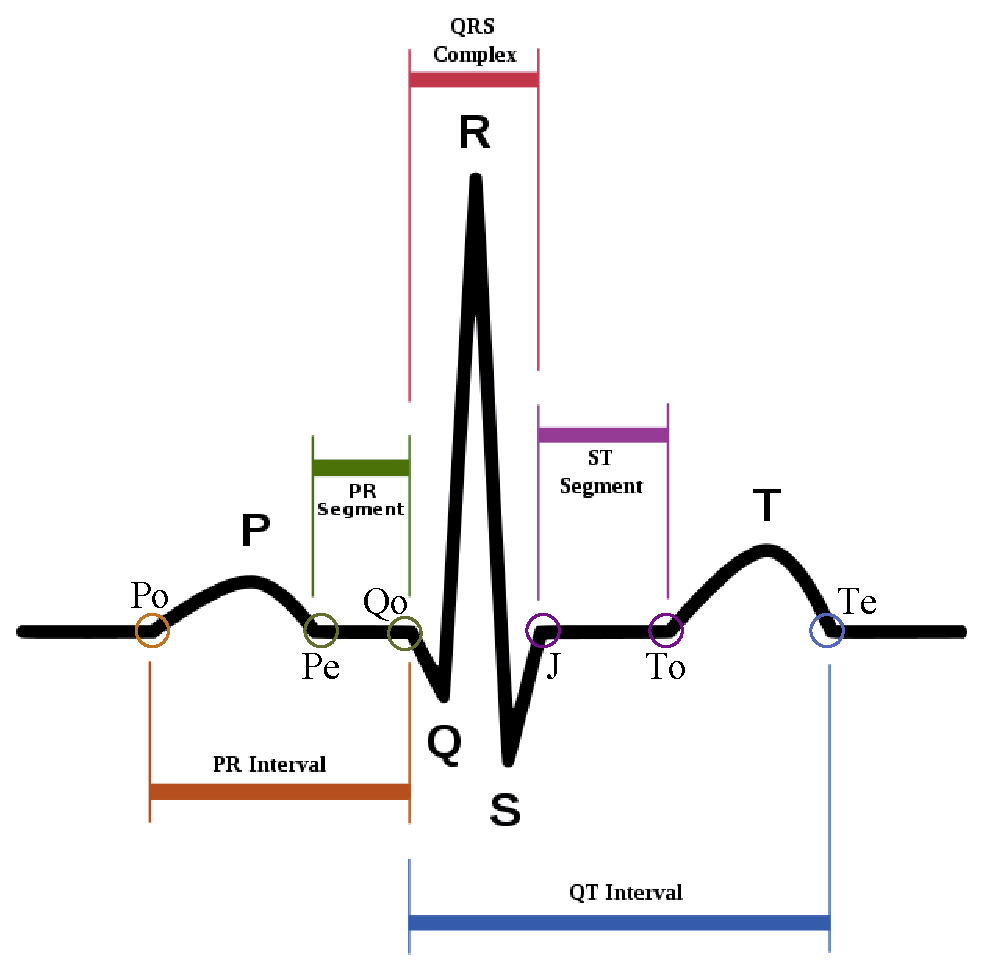
\includegraphics[height=3.0in]{./Figure/rr_interval_label.eps}
\caption{Standard ECG with labels.}
\label{fig_ECG_lable}
\end{figure}


Considering these properties, we propose an ECG-oriented metric, which defines how to measure the dissimilarity between two unequal-lengthed PT intervals.


\textbf{Stream clustering algorithm:}


Different from the clustering of unchanged data, stream clustering poses several additional requirements: under the stream clustering scenario, data will arrive continuously, which means that the algorithm has to generate results in a very limited time. Moreover, the undergoing changes may cause existing clusters to emerge, merge and split, so the algorithm should be aware of these changes.


In our work, we introduce a new stream clustering algorithm for ECG stream data and empirically demonstrate its practical performance. The key idea of our algorithm is that as the new data arrives, it is clustered into several new clusters without initially taking the existing data into account. The connectivity and distortion of these new clusters and existing clusters will then be evaluated globally. Those clusters which have high connectivity would be merged into one, and the clusters which have high distortion would be divided into smaller clusters. This approach iterates as new batch of data comes in.


\textbf{Speeding up with MapReduce:}


To conquer the challenge derived from scaling our system over massive data, we choose to implement our system on top of MapReduce. MapReduce is actually a framework for processing sophisticated parallel problems, in which the Map is used to execute independent computation on a part of the data in parallel while the Reduce is responsible for ''summing up'' the result of the Map. However, due to the inherent nature of our workflow, not all the computation could be distributed, thus deciding which part to distribute becomes a vital issue for our system performance.


To improve the performance as much as possible, we carefully design our workflow according to the MapReduce model in order to distribute most of the computation among the cluster. For some parts of the workflow which are dependent on the others, we break them into smaller granularity and try to execute the independent parts in parallel and run the dependent parts in sequence.



\section{ECG-Oriented Metric}
As mentioned in section II, the primary step of cluster analysis is to define the basic processing unit. In our system, the PT interval is used as the basic unit of clustering. So, as soon as a batch of ECG data arrives, a conventional wavelet transformation based algorithm is applied to find the feature points. According to these feature points, the ECG data could easily be interpreted into PT intervals.

After that, we define how to measure the dissimilarity between these basic processing units. Considering the special properties of PT intervals, this is not easy work.


The primary challenge deriving from the special properties of PT interval is that they are time series data of unequal length. This makes some conventional metrics like Euclidean metrics inapplicable since they could only handle data of equal length. So, to measure the dissimilarity between PT intervals properly, we first align these PT intervals by adopting the Dynamic Time Warping (DTW) algorithm \cite{sakoe1978dynamic}: Given two sequences of time series data $ M $ and $ N $, with length $ m $ and $ n $ respectively, the DTW algorithm would yield an optimal warping path between the two data by using the dynamic programming approach. The warping path $  WP $ is a set of tuples which is defined below:
\begin{equation}
WP = \{ (i, j) \; | \; 0 \leq i \leq m, \; 0 \leq j \leq n  \}
\end{equation}
where each tuple $ (i, j) $ in the warping path implies that the $ i^{th} $ element in the data $ M $ should be aligned with the $ j^{th} $ element in the data $ N $. So, with this warping path, these two time series data $ M $ and $ N $ could be aligned easily.


Another issue raised from the special properties of PT interval is that considering the nature of ECG, some regions of the PT interval are more important than others. Taking this into account, we divide the PT interval into three segments and assign each segment with a heuristic weight, that is:
\begin{equation}\label{PT_segment}
\left\{ \begin{array}{ll}
s_1 = [P_o, Q_o], \; w_1 = 0.15\\
s_2 = [Q_o, J], \;  w_2 = 0.5\\
s_3 = [J, T_e], \; w_3 = 0.35
\end{array} \right.
\end{equation}
where the $ P_o $ is the beginning point of P wave, $ Q_o $ is the beginning point of Q wave, $ J $ is the end point of S wave, the $ T_e $ is the end point of T wave, and the $ w_1 $, $ w_2 $ and $ w_3 $ is the heuristic weight of each segment respectively. All of these points are shown in Figure \ref{fig_ECG_lable}.


Combining these two ideas, we get the procedure of measuring the dissimilarity between PT intervals: Firstly, a standard PT interval would be synthesized, and all of the PT intervals, including the synthesized one, would be divided into three segments: $ s_1, s_2, s_3 $ according to the equation (\ref{PT_segment}). Then, the DTW algorithm is applied between each PT interval and the standard PT interval on $ s1 $, $ s2 $ and $ s3 $ respectively to find the warping paths. By aligning the $ s_1 $, $ s_2 $ and $ s_3 $ respectively, all the PT intervals would be aligned with the standard PT interval. After that, the dissimilarity between two PT intervals can be defined as the sum of the weighted Euclidean distance of the aligned segment. 


That is, given two PT intervals $ Q $ and $ R $, which have been aligned with the standard PT interval, the dissimilarity $ Dis(Q, R) $ between these two PT intervals is defined as:
\begin{equation}\label{eq_dissimilarity}
Dis(Q, R) = \sum_{i=1,2,3}{w_i * dis(s_{iq}, s_{ir} )}
\end{equation}
where $ s_{iq} $ and $ s_{ir} $ are the aligned segments $ i $ in $ Q $ and $ R $ respectively, and the $ dis(X, Y) $ is the Euclidean distance between equal-length data $ X $ and $ Y $.

\begin{figure}[!t]
\centering
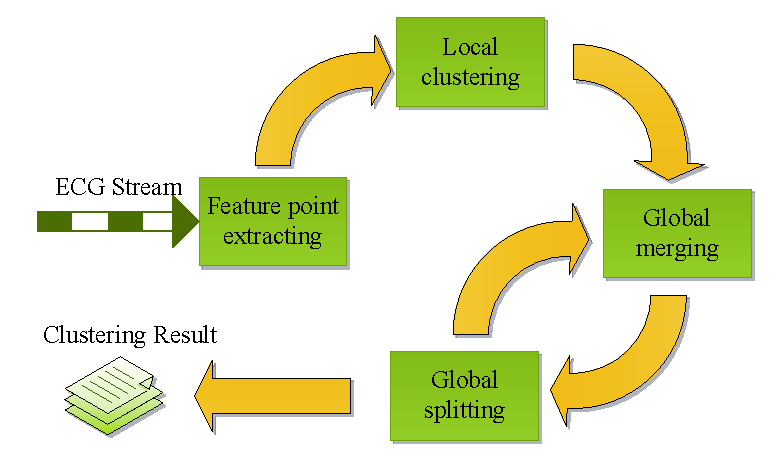
\includegraphics[height=2.0in]{./Figure/algorithm_overview.eps}
\caption{Algorithm overview.}
\label{fig_algorithm_overview}
\end{figure}

\begin{figure*}[!t]
\centering
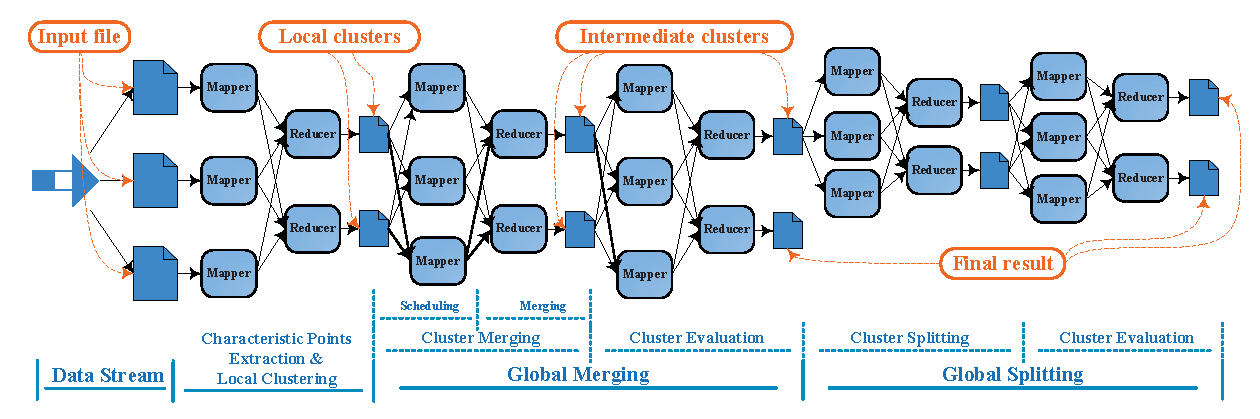
\includegraphics[width=7.1in]{./Figure/system_overview.eps}
\caption{The overview of system.}
\label{fig_sys_overview}
\end{figure*}
\section{Stream Clustering}
% the brief step of whole algorithm
% the detail of each
The design preference of providing continuous monitoring services in the ECG telehealth system has made the data arrive in the system as a stream with high update rate. This nature of this stream requires the clustering algorithm not only to be able to generate results in a limited time but also be aware of the undergoing changes. Under these concerns, we present our stream clustering algorithm, which could generate results in an incremental manner by dynamically merging and splitting clusters. Figure \ref{fig_algorithm_overview} gives an overview of the whole clustering algorithm. In this approach, as a batch of ECG stream data arrives, an iteration of clustering would be triggered and the whole iteration can be divided into three steps: local clustering, global merging and global splitting.


Step 1 is called local clustering. In this step, the ECG data has already been interpreted into PT intervals, and these PT intervals would be divided into several groups randomly and uniformly. Then, for each group, a K-Means algorithm is applied to generate $ k $ clusters respectively, where the parameter $ k $ is used to control the granularity of local clustering. After the clustering, the cluster features of each cluster would be computed, the cluster feature $ CF $ is actually the representation of a cluster, which is defined as below:
\begin{equation}
CF(C) = (c, \; e, \; r, \; lr)
\end{equation} 
where the $ c $ is the centre of cluster $ C $, $ e $ is the centre of the Euclidean space, $ r $ is the average distance between centre $ c $ and the PT intervals in this cluster, and the $ lr $ is the maximal distance between centre $ c $ and the PT intervals in the cluster. 

%They are defined mathematically as bellow:
%\begin{equation}\label{eq_CF_defination}
%\left\{ \begin{array}{ll}
%c = argmin \; \{ \sum\limits_{p_i \in C}{Dis(p_i, c)} \}  \\
%e = \{ (e_1, e_2, ..., e_n) | e_j = [max(p_{ij}) + min(p_{ij})] / 2  \}, \\
%r = [ \, \sum\limits_{p_i \in C}{Dis(p_i, c)} \, ] / n \\
%lr = max \; \{ Dis(p_i, c) \}
%\end{array} \right.
%\end{equation}
%where $ n $ is the number of points in cluster $ C $

Some PT intervals that should belong to the same cluster,  might be divided into different groups and thus be clustered separately which eventually leads to their misplacement. A global merging and splitting is performed after the local clustering to address this problem. 


Step 2 is the global merging. In this phase, we first define the connectivity $ con $ between two clusters $ Q $ and $ T $ as below:
\begin{equation}\label{eq_connectivity}
con(Q, T) = \frac{(r_q + r_t)}{Dis(c_q, c_t)} 
\end{equation}
where the $ r_q $ and $ r_t $ is the average radius $ r $ of cluster $ Q $ and cluster $ T $, the $ c_q $ and $ c_t $ is the centre of cluster $ Q $ and $ T $, and $ Dis(c_q, c_t) $ is the dissimilarity measurement between $ c_q $ and $ c_t $


All the connectivity between each pair of clusters generated by the local clustering and existing clusters which are generated by the previous iterations would be calculated. After that, all the cluster pairs whose connectivity is satisfied the following condition would be merged into one cluster:
\begin{equation}\label{eq_mergingCondition}
con(Q, R) \geq \lambda
\end{equation}
where $ \lambda $ is a pre-defined parameter to control the granularity of global merging.


Although the global merging would redress the misplacement caused by local clustering, but it also might degrade the cluster quality by merging heterogeneous clusters together. So after the global merging, a cluster evaluation would be performed on each cluster generated from global merging to evaluate the quality of the clusters. The quality of a cluster is represented by its distortion error, and the evaluation function of distortion error is defined as below:
\begin{equation}\label{eq_quality}
DST(C) = \frac{w_1 * r + w_2 * Dis(c, e )}{lr}
\end{equation}
where the $ DST(C) $ is the distortion error of cluster $ C $, the $ w_1 $ and $ w_2 $ is the heuristic weight which empirically set to be $ 0.3 $, $ 0.4 $ respectively in our system, the $ r $ is the average distance of cluster $ C $, the $ c $ is the centre of cluster $ C $, the $ e $ is the centre of Euclidean space, and $ Dis(c, e) $ is the dissimilarity measurement between $ c $ and $ e $. 


After the cluster evaluation, all the clusters which satisfy the following splitting condition would be applied with a K-Means algorithm to split into two smaller clusters:
\begin{equation}\label{eq_splittingCondition}
DST(C) \geq \tau
\end{equation} 
where $ \tau $ is a pre-defined parameter to control the granularity of global splitting. 


After the global splitting, the whole clustering iteration ends. The final clustering result is saved in the file system in order to cluster newly arrived data incrementally in the next iteration.


\section{Speedup with MapReduce}
The data we are processing is stream data with high update rate, which implies that the data volume in our system would increase exponentially as time goes by. To handle such massive data properly, we implement our system on top of the MapReduce framework. For better utilization of the power of MapReduce, we designed our system workflow carefully in order to distribute as much computation as possible. Figure \ref{fig_sys_overview} shows the workflow of our system on top of MapReduce.


In this workflow, as the workload of feature point extraction is relatively lightweight, it has been combined into the local clustering step. It is obvious that the job of both feature point extraction and local clustering are independent of each others, so it would be easily distributed by performing the job in the MAP.


However, the situation becomes more complex when it comes to global merging. As it would cross check all the clusters to calculate the connectivity, global merging seems to be unable to distribute among clusters. After carefully investigating the workflow of global merging, we have found that this step could be divided into two smaller steps: generating merging plan and merging. The first step would calculate the pair-wise connectivity between clusters to generate a merging plan. Due to its serial nature, this step would only be able to run in sequence. Meanwhile, the second step conducts the actual merging according to the merging plan assigned to it and updates the cluster feature for new clusters. As it only concerns the data contains in the merging plan, this step could be performed in MAP and run in parallel 


In the global merging, we actually have two MapReduce jobs: one for global merging and another one for cluster evaluation. Although the latter would only update the cluster feature for newly-generated clusters, it would not be combined with the previous MapReduce job. Recall that for new clusters, we have to calculate the centre and the average radius of cluster. This requires to scan over the whole data twice at least, the first one finds the centre, and the next one calculates the average radius with respect to the centre. However, this could not be done in a single REDUCE, because there is only one iteration allowed in the REDUCE as considering the input data, the volume of REDUCE would be extremely large. As a result, the latter MapReduce job for cluster evaluation is inevitable.

For the global splitting, as it only concerns a part of the whole data and is thus independent of the others, this step could be distributed easily. As mentioned before, an inevitable cluster evaluation job would be performed after the global splitting.

\section{Evaluation}
We implemented our system on top of Hadoop 0.20.2. As described in the previous section, this system consists of multiple MapReduce jobs, and all the jobs are implemented in Java. To prepare the data for evaluation, we cooperate with New Element Medical Ltd.,Co, Shenzhen, China, which provides us a real ECG database collected from hundreds of users, including users of different age, gender and heart status. In the database, there are more than 1,500 ECG data files, each of which contains about 2,800 PT intervals. So, approximately, there are 4,356,800 PT intervals in total. With these data, we conduct our evaluation on a homogeneous Hadoop cluster, in which each node runs a CentOS release 5.5 and is equipped with an Intel Xeon CPU X3430 @ 2.4 GHz with 4 cores, 4 GB of RAM and 160 GB of hard disk. For all the experiments, we set the parameters in our system as below:
\begin{equation}
\{ k=4, \; \lambda=1.0, \; \tau=0.4 \;  \}
\end{equation}
where $ k $, $ \lambda $ and $ \tau $ are the parameter which control the granularity of local clustering, global merging and global splitting respectively.


For the evaluation, we first conduct a baseline performance evaluation, in which we cluster an ECG stream consisting of 1500 ECG data files and report the clustering result. Then, the scalability characteristic of our system with respect to the number of computing cores is evaluated. Apart from this, we also evaluate the performance of our system with respect to different block size of HDFS. 

\textbf{Baseline performance evaluation:}


In this evaluation, we use our system to cluster an ECG stream consisted of all the ECG data files from the real ECG database. The whole data is clustered into 4 clusters and some important statistics of each cluster are listed in table \ref{tb_clustering_result}, where the cluster size is the number of PT intervals in the cluster, the total distance is the sum of distances between the cluster centre and the PT intervals in the cluster, the average radius is the average distance between the cluster centre and the PT intervals in the cluster, and the maximal radius is the maximal distance between the cluster centre and the PT intervals in this cluster. To provide an intuitive view of the clustering results, Figure \ref{fig_clustering_result} plots all the PT intervals belong to the last cluster in the clustering result by overlapping them in a single figure.
\begin{table}[!t]\caption{Clustering Result}
\label{tb_clustering_result}
\centering
\begin{tabular}{|c|c|c|c|c|}
\hline
ID & Cluster size & Total distance & Average radius & Maximal radius\\
\hline
C1 & 2753836 & 130889825.08 & 47.53 & 186.50 \\
C2 & 1922412 & 107558951.40 & 55.95 & 202.10 \\
C3 & 2003 & 55743.49 & 27.83 & 88.04 \\
C4 & 11771 & 289684.31 & 24.61 & 110.13 \\
\hline
\end{tabular}
\end{table}

\begin{figure}[!t]
\centering
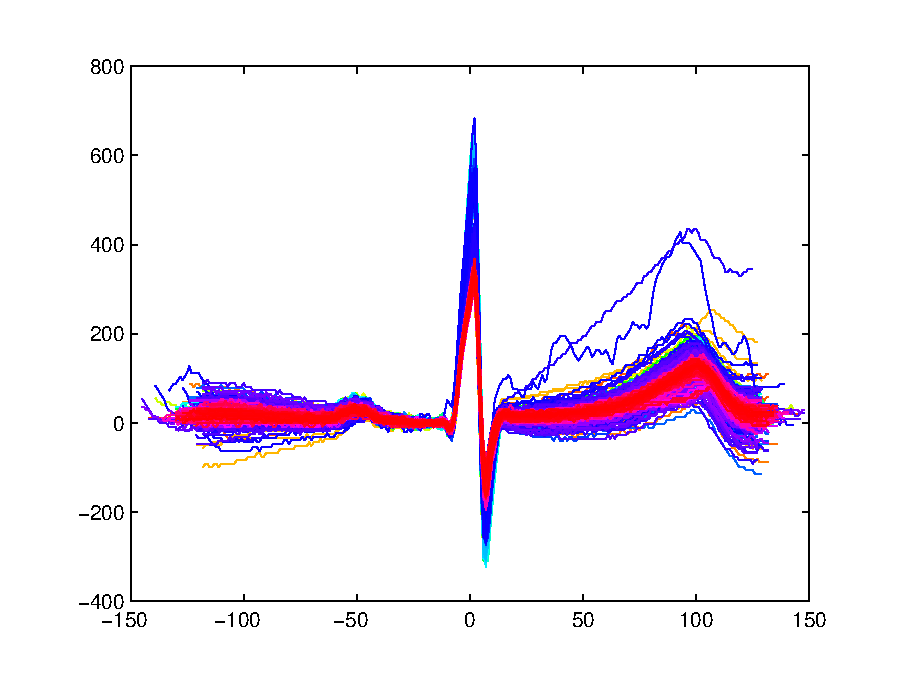
\includegraphics[height=2.5in]{./Figure/cluster_result.eps}
\caption{One of the clustering results.}
\label{fig_clustering_result}
\end{figure}

\textbf{Scalability with computing cores:}


To evaluate the scalability of our system, we conduct an experiments which processes 300 ECG data files in each iteration of clustering and run this experiment on a cluster scale from 8 cores to 32 cores (each node in our cluster has 4 cores, and there are 8 nodes in total). Figure \ref{fig_scalability_total_cores} shows the average running time of our system with different number of computing cores. It is obvious that the total running time is decreasing significantly as the number of computing cores grows, which shows that our system scales well on multiple computing cores. 


The average running of each step of our stream clustering algorithm is also evaluated. As showed in Figure \ref{fig_scalability_phase_cores}, we have found that the global merging is the most time consuming job in the whole process. This is because the workload is quite heavy since it has to cross check all the existing clusters in a serial manner and when it executes the actual merging work, it causes a lot of IO operations. We also notice that the global merging benefits significantly when increasing the number of cores. This could be explained by observing the fact that the most work in the global merging are done in the reduce stage. Since the number of reducers is relative to the number of computing cores, there would be more reducer running in parallel as the number of computing cores grow, which could speed up the global merging significantly.

\begin{figure}[!t]
\centering
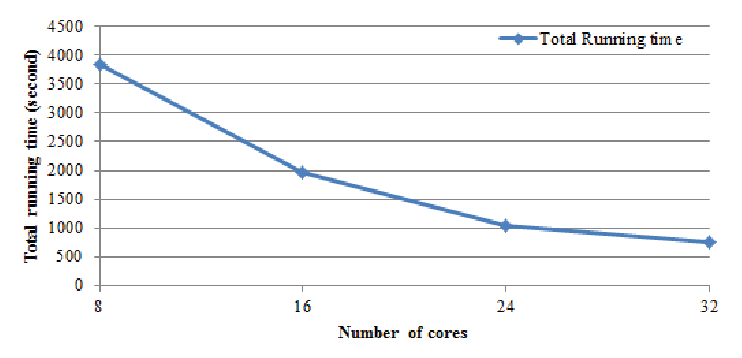
\includegraphics[height=2.0in]{./Figure/runningTime_cores.eps}
\caption{Scalability of PESC system.}
\label{fig_scalability_total_cores}
\end{figure}

\begin{figure}[!t]
\centering
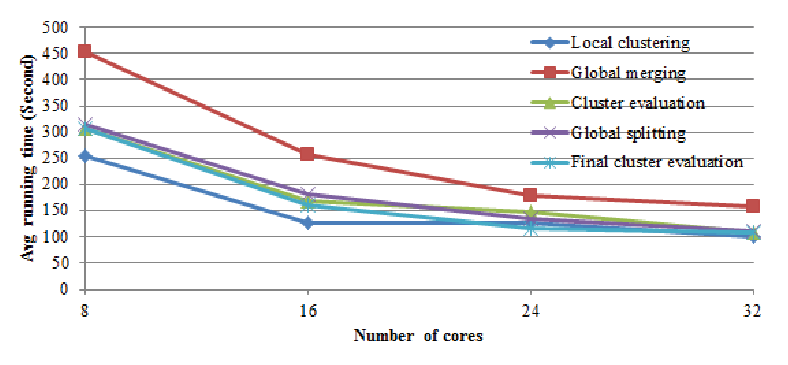
\includegraphics[height=1.8in]{./Figure/phase_cores.eps}
\caption{Scalability of steps in stream clustering algorithm.}
\label{fig_scalability_phase_cores}
\end{figure}

\textbf{Optimization with block size: }


As mentioned at the beginning of this section, the database we are using consists of thousands of small files. However, processing large volumes of small files in Hadoop could be quite frustrating. One of the most significant reasons is that for each file in the HDFS which is smaller than a block would still occupy a block. That is, as the default block size of HDFS is 64 MB, if there are 10,000 files in HDFS, each of which is smaller than 64 MB, then these files will occupy $ 10,000 * 64 MB = 625 GB $ in the HDFS, which would degrade the performance significantly. To evaluate the influence of block size to our system performance, we run our system with different block size and the result is shown in Figure \ref{fig_block_size}. It is found that when the block size of HDFS is significantly larger than the size of the files stored in it, the total running time is quite high since there are lots of useless IO and network overheads. However, due to the fact that each map task usually processes a block of input at a time, if the block size are noticeable smaller than the input files size, then there will be plenty of map tasks, each of which imposes extra bookkeeping overhead, which eventually degrades the performance.
\begin{figure}[!t]
\centering
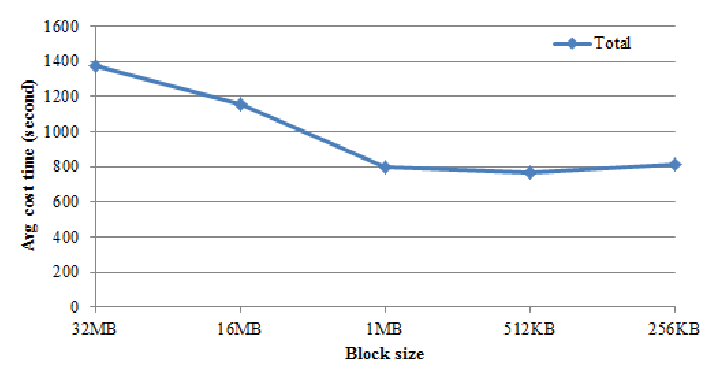
\includegraphics[height=2.0in]{./Figure/block_size.eps}
\caption{PESC performance V.S. HDFS block size.}
\label{fig_block_size}
\end{figure}



\section{Conclusion}
We have designed and implemented the PESC, a parallel system for massive ECG stream clustering. Our system would perform the clustering by adopting an ECG-oriented metric and try to achieve the global optimum by merging and splitting dynamically. The evaluation result shows that our system would not only provide a good clustering result but also produces an excellent performance on multiple computing nodes.





% conference papers do not normally have an appendix


% use section* for acknowledgement
%\section*{Acknowledgement}




% trigger a \newpage just before the given reference
% number - used to balance the columns on the last page
% adjust value as needed - may need to be readjusted if
% the document is modified later
%\IEEEtriggeratref{8}
% The "triggered" command can be changed if desired:
%\IEEEtriggercmd{\enlargethispage{-5in}}

% references section

% can use a bibliography generated by BibTeX as a .bbl file
% BibTeX documentation can be easily obtained at:
% http://www.ctan.org/tex-archive/biblio/bibtex/contrib/doc/
% The IEEEtran BibTeX style support page is at:
% http://www.michaelshell.org/tex/ieeetran/bibtex/
%\bibliographystyle{IEEEtran}
% argument is your BibTeX string definitions and bibliography database(s)
%\bibliography{IEEEabrv,../bib/paper}
%
% <OR> manually copy in the resultant .bbl file
% set second argument of \begin to the number of references
% (used to reserve space for the reference number labels box)

\bibliographystyle{IEEEtran}
\bibliography{IEEEabrv,./ECG_Stream_Clustering_with_MapReduce}



% that's all folks
\end{document}


